\section{COMPONENTE CLIENTE}

El componente cliente se ha implementado utilizando varias tecnologías web:

    \begin{itemize}

        \item PHP

            El cliente se encuentra desarrollado en la misma aplicación servidora. De esta manera, las sesiones de usuario son compartidas por lo que hay una mayor facilidad de integración, y por otro lado se facilita la instalación en un único servidor.

            La única funcionalidad que se utiliza es la comprobación de la sesión de un usuario, pintando en un caso la página pública o en otro la zona privada. Estas son las dos únicas páginas que renderiza el servidor, a partir de ahí el cliente es quien pide la información vía peticiones \emph{RESTful} en formato \emph{JSon} y renderiza la web a través de las plantillas con \emph{handlebars}.

        \item HTML

            Es un lenguaje de marcas de hipertexto (\emph{HyperText Markup Language}) que permite definir la estructura y el contenido de una página web (texto, imágenes, hipervínculos...). Es un estándar que regula la W3C (\emph{World Wide Web Consortium}) que todos los navegadores intentan cumplir, de manera que el contenido HTML de la página se visualice de la manera más parecida en los distintos navegadores.

        \item CSS

            Es un lenguaje de hojas de estilo (\emph{Cascading Style Sheets}) que permite definir el aspecto y el formato de un documento escrito en un lenguaje de marcas, como HTML, y al igual que este las especificaciones están reguladas por el consorcio de la \emph{W3C}.

        \item Bootstrap

            Es un framework CSS que define unas reglas de estilos para estructurar el diseño de la página web. Está desarrollado por \emph{Twitter} el cual ha publicado el código bajo la licencia \emph{MIT}.

        \item JavaScript

            Es un lenguaje de programación interpretado, dinámico y normalmente usado en páginas web que corren bajo un navegador web. Aunque, también se puede utilizar desde el lado de servidor a través de tecnologías como \emph{Node.js}.

            Desde el lado del cliente a través del navegador permite:

                \begin{itemize}
                    \item Interactuar con el usuario.
                    \item Controlar el navegador.
                    \item Realizar comunicaciones asíncronas con el servidor (\emph{AJAX}).
                    \item Alterar el contenido del documento que se está visualizando.
                \end{itemize}

        \item Handlebars

            Es una librería JavaScript para la creación de plantillas, las cuales son compiladas y reciben un objeto JSon con los datos, siendo procesado por \emph{Handlebars} para obtener el documento HTML.

        \item JQuery

            Es una librería JavaScript que simplifica el manejo del documento HTML (manipulación, eventos, animaciones, Ajax...). Además, ofrece compatibilidad con la mayoría de los navegadores del mercado.

        \item Director

            Es una librería JavaScript que simplifica la creación de rutas enfocado a webs de una única página, donde toda la información se carga vía Ajax y plantillas. Utiliza la HTML5 History API para manipular la URL del navegador sin recargar la página entera, dando la sensación de navegación entre distintas páginas web.

    \end{itemize}

Se han creado dos zonas web diferenciadas; una parte pública donde el usuario puede loguearse o registrarse en el sistema; y una parte privada donde el usuario puede acceder a su información.

La zona privada de la plataforma web se ha creado utilizando un diseño conocido como Single Page App, es decir, se carga la página una sola vez y toda la navegación posterior se realiza mediante \emph{Ajax} y un sistema de plantillas.

Las ventajas de este diseño es que no es necesario recargar la página entera cada vez que se quiere acceder a una nueva sección, solo se necesitan pintar pequeñas zonas de la página web. Una de las desventajas es que las páginas que se crean con este diseño no son facilmente indexadas por los buscadores, por ello, es un diseño que se suele utilizar en zonas privadas donde no tienen acceso a los buscadores y no importa que el contenido no sea indexado.

\subsection{Flujo de la aplicación}

    A continuación se muestra un diagrama con el flujo por las distintas páginas de la aplicación web y las acciones que se pueden realizar en cada una de ellas.

    \begin{figure}[H]
        \centering
        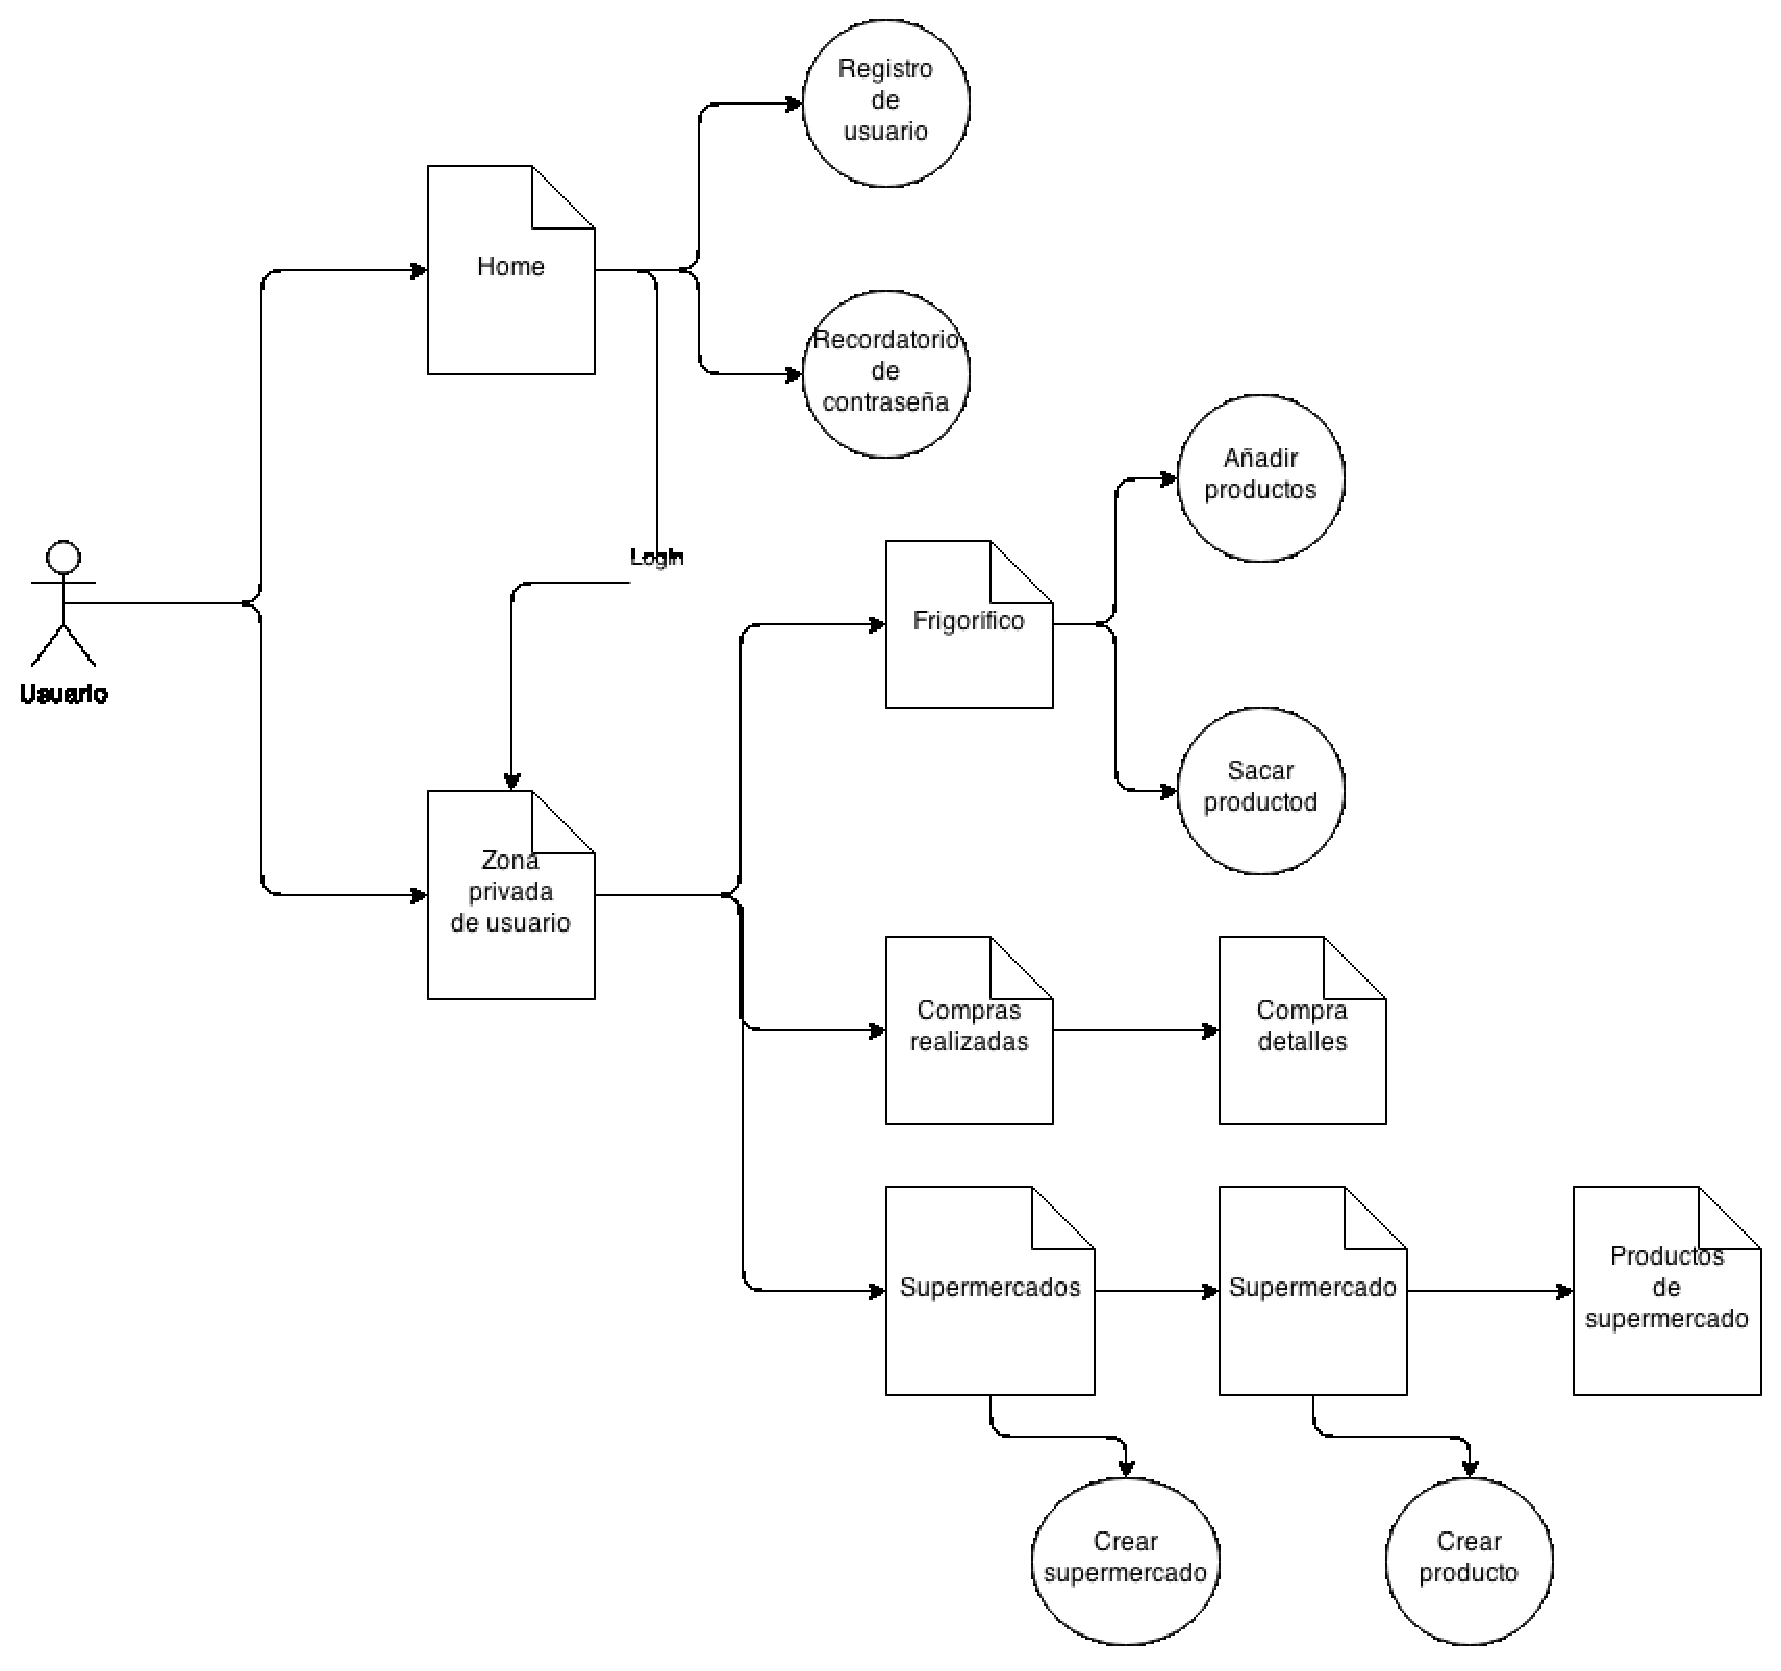
\includegraphics[keepaspectratio,width=0.9\textwidth]{flujo-aplicacion-web.eps}
        \caption{Flujo de la aplicación web}\label{fig:flujo-aplicacion-web}
    \end{figure}
